\documentclass[tikz,border=2pt]{standalone}
\usepackage{amsmath,amssymb}
\usepackage{pgfplots}
\pgfplotsset{compat=1.18}
\usetikzlibrary{arrows.meta}
\begin{document}
% Tail-sum form of the expected backlog, Lighthouse lead-time demand (l = 2), S = 8:
% E[I^-] = sum_{j >= 8} G_X(j) = G_X(8) + G_X(9) = 31/360 = 0.086; the bars j < 8 sum to 4.464,
% all bars sum to E[X] = 4.55.
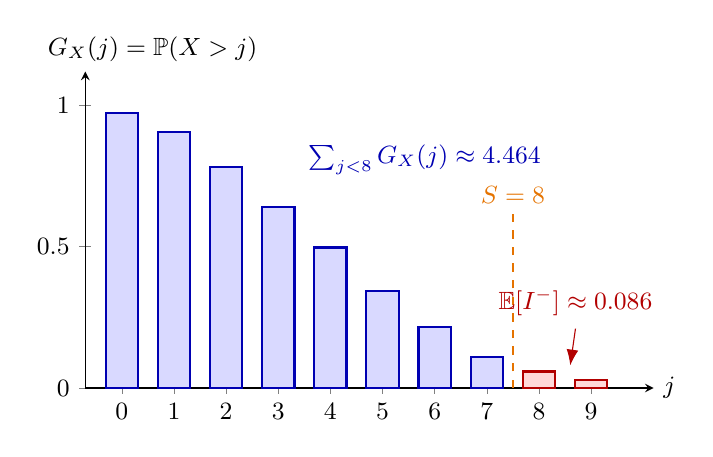
\begin{tikzpicture}[font=\small, >={Latex[length=2mm]}]
  \begin{axis}[axis lines=left, xmin=-0.7, xmax=10.2, ymin=0, ymax=1.12,
    xtick={0,...,9}, ytick={0,0.5,1}, yticklabels={$0$,$0.5$,$1$},
    xlabel={$j$}, ylabel={$G_X(j)=\mathbb{P}(X>j)$},
    xlabel style={at={(axis description cs:1,0)}, anchor=west},
    ylabel style={rotate=-90, at={(axis description cs:0,1)}, anchor=south west, xshift=-6mm},
    width=8.8cm, height=5.6cm, clip=false]
    \addplot[ybar, bar width=0.62, fill=blue!15, draw=blue!70!black, thick]
      coordinates {(0,0.9722) (1,0.9056) (2,0.7822) (3,0.6406) (4,0.4975) (5,0.3428) (6,0.2147) (7,0.1084)};
    \addplot[ybar, bar width=0.62, fill=red!15, draw=red!70!black, thick]
      coordinates {(8,0.0583) (9,0.0278)};
    \draw[orange!90!black, thick, dashed] (axis cs:7.5,0) -- (axis cs:7.5,0.62);
    \node[orange!90!black, anchor=south] at (axis cs:7.5,0.62) {$S=8$};
    \node[blue!70!black, anchor=south west] at (axis cs:3.4,0.72) {$\sum_{j<8}G_X(j)\approx4.464$};
    \node[red!70!black, anchor=south] at (axis cs:8.7,0.22) {$\mathbb{E}[I^-]\approx0.086$};
    \draw[red!70!black, thin, ->] (axis cs:8.7,0.21) -- (axis cs:8.6,0.08);
  \end{axis}
\end{tikzpicture}
\end{document}
